\documentclass[11pt]{article}
\usepackage[utf8]{inputenc}
\usepackage{amsmath,amssymb,amsthm}
\usepackage{graphicx}
\usepackage[margin=1.1in]{geometry}
\usepackage{hyperref}

\newtheorem{theorem}{Theorem}
\newtheorem{lemma}[theorem]{Lemma}
\newtheorem{proposition}[theorem]{Proposition}
\newtheorem{corollary}[theorem]{Corollary}
\newtheorem{conjecture}[theorem]{Conjecture}
\theoremstyle{definition}
\newtheorem{definition}[theorem]{Definition}
\newtheorem{remark}[theorem]{Remark}
\newtheorem{openproblem}[theorem]{Open Problem}

\newcommand{\lexmax}{\mathrm{lexmax}}
\newcommand{\R}{\mathbb{R}}

\title{Greedy Packing of Nested Rings:\\ Superadditivity, Placement Rules, and a Tribonacci Threshold}
\author{Javier Aguilar Mart\'in\thanks{Independent researcher.
\texttt{javier.aguilar@sapira.ai}. Computational verification scripts for
every numerical claim, together with extended proofs and the verification
reports cited in the appendix, are available in the accompanying repository,
\url{https://github.com/JaviMaligno/calamares} (\texttt{python
code/run\_all.py} reproduces every verification; the arXiv version will pin
the exact commit).}}
\date{\today}

\begin{document}
\maketitle

\begin{abstract}
We study packings of annuli (``rings'') of common width into a disk, where
a ring may nest inside the hole of a strictly larger one -- a circular,
selection-oriented relative of the Recursive Circle Packing Problem. The
two natural objectives, number of placed rings and total contact area,
genuinely diverge: area is a superadditive function of the radius,
cardinality is not. For \emph{superincreasing} radii (each exceeding the
sum of all smaller ones) we prove that the descending greedy maximizes
every positive, strictly increasing, superadditive objective, and -- our
main structural theorem -- that the placement rule is irrelevant: any
choice among feasible containers yields the lexicographically maximal
feasible set, for containers of arbitrary shape and in every dimension.
Both hypotheses are sharp: placement irrelevance holds unconditionally for
at most three rings and fails at four, and \emph{twin instances} rule out
every placement rule that is a function of the observable state. Measuring
the violation of superincreasingness by $\rho=\max_i(\sum_{j>i}r_j)/r_i$,
the additive relaxation of the model has universal threshold exactly
$\rho=1$, while the geometric model resists further: we prove, with no
tangency idealization, that the four-ring rigid family of counterexamples
has infimum exactly the Tribonacci constant $T\approx1.83929$, and we
conjecture that the geometric threshold is exactly $T$. We develop a
supporting program towards the conjecture -- exact positive-width curves
with global minimum $13/7$, closed profile thresholds, and blocking walls
for generic containers with metallic-mean floors -- and complement it with
a phase diagram for the divergence of the objectives and a decoupling of
hardness into a geometric layer and a combinatorial (subset-sum) layer, of
which superincreasingness eliminates exactly the latter.
\end{abstract}

\section{Introduction}

Drop a batch of squid rings into a frying pan and a natural optimization
problem appears: place as many rings as possible flat on the pan -- or, if one
cares about searing, maximize the total ring--pan contact area -- exploiting the
fact that a sufficiently small ring fits inside the hole of a larger one.
Abstracted, this is the problem of packing annuli of common width into a disk
with recursive nesting, a circular-container relative of the
\emph{Recursive Circle Packing Problem} (RCPP) introduced by Pedroso, Cunha and
Tavares~\cite{PedrosoCunhaTavares2016} to model the ``telescoping'' of tubes in
shipping containers, and attacked exactly by Gleixner, Maher, M\"uller and
Pedroso~\cite{Gleixner2020}. That literature is algorithmic: it packs a fixed
set of rings into as few rectangular containers as possible. Here we ask
structural questions instead: which objectives does the natural greedy
algorithm optimize, when is the choice of \emph{where} to put each ring
irrelevant, and what conditions on the radii govern the answers.

Our starting point is a classical phenomenon in one dimension. For bin packing
with \emph{divisible} item sizes, Coffman, Garey and
Johnson~\cite{CoffmanGareyJohnson1987} proved that First Fit Decreasing is
optimal. We are not aware of an analogue for geometric packing of disks, let
alone with nesting. We prove one, with \emph{superincreasing} radii (each radius exceeding
the sum of all smaller ones) playing the role of divisibility, and we determine
exactly how far the hypothesis can be relaxed -- with a surprising answer: the
additive relaxation of the model has threshold exactly $1$, while the geometric
model resists up to (conjecturally, exactly) the Tribonacci constant.

\paragraph{Contributions: main theorems.}
(1)~A \emph{superadditivity dichotomy}: under superincreasing radii the
selection greedy is optimal for every positive, strictly increasing,
superadditive value function of the radius -- contact area is one -- while
cardinality (not superadditive) admits counterexamples even under
superincreasing radii (Section~\ref{sec:superadd}). The selection statement
is best seen as a general fact about downward-closed set systems with
superincreasing weights, in the lineage of greedy analyses on independence
systems~\cite{Edmonds1971,KorteHausmann1978} and of the superincreasing
knapsack~\cite{Gupte2016}; the geometric content of this paper begins with
the next item.
(2)~A \emph{placement-obliviousness theorem}: under superincreasing radii,
\emph{any} rule for choosing among feasible containers yields the
lexicographically maximal feasible set; the proof is container-shape- and
dimension-agnostic (Section~\ref{sec:oblivious}).
(3)~\emph{Sharpness}: placement obliviousness holds unconditionally for
$n\le3$ rings and fails at $n=4$; twin instances with an identical prefix rule
out every state-based placement rule, deterministic or randomized
(Section~\ref{sec:sharp}).
(4)~\emph{Thresholds}: the additive model has universal threshold exactly
$\rho=1$; the geometric four-ring rigid subfamily has infimum exactly the
Tribonacci constant $T$, proved with no idealization
(Theorem~\ref{thm:rigidfloor}, full proof in
Appendix~\ref{app:rigidproof}), and we conjecture the geometric threshold
equals $T$ (Section~\ref{sec:threshold}).

\paragraph{Contributions: the program towards the Tribonacci threshold.}
(5)~\emph{The width program}: the blocked-exchange infimum with relative
width $\omega>0$ is governed by the deformed Tribonacci cubic
$\alpha^3=(1+\omega)(\alpha^2+\alpha+1)$; the full lower-bound curve is in
closed form and its global minimum is exactly $13/7$, attained at a rational
corner (Section~\ref{sec:width}); the combinatorial profile threshold is
closed for every profile size, with golden plateau and exact Tribonacci
crossing $\omega_T=1/T-1/2$.
(6)~\emph{Generic containers}: an exact corona criterion for wall-tangent
packings (with two corrective counterexamples and a $k=5$ ``pentagram''
certificate), and a hierarchy of blocking walls -- occupant holes, ``blocking
costs the slack'', and the double pocket -- yielding metallic-mean floors
(silver ratio $1+\sqrt2$, golden line $\varphi^2-(\varphi/2)\omega$) that
push every blocked exchange with extra occupants above $T$ -- for all widths
$\omega<0.9626$ with one extra occupant, up to $0.624$ and $0.896$ with two
and three, and for all widths with four or more
(Section~\ref{sec:generic}). The remaining gaps of the program are stated
explicitly there and in Open Problem~\ref{op:assembly}.
(7)~A phase diagram for the divergence of the two objectives, and a
decoupling of hardness into a geometric and a combinatorial layer, the
latter with an explicit \textsc{Partition} reduction
(Sections~\ref{sec:divergence}--\ref{sec:hardness}).

\section{Model and preliminaries}\label{sec:model}

\begin{definition}[Rings and placements]
Fix a width $w>0$. A \emph{ring} of outer radius $r>0$ is an annulus with
inner (hole) radius $\max(0,\,r-w)$; if $r\le w$ it is a solid disk with no
hole. Let $K\subset\R^d$ be a compact \emph{container} (the \emph{pan}; our
motivating case is a disk of radius $R$ in the plane, $d=2$, but
Theorems~\ref{thm:selection} and~\ref{thm:oblivious} hold for arbitrary $K$ and
$d$, with rings read as spherical shells). A \emph{placement} of a subset $S$
of the rings is a forest: each placed ring has as parent either the pan or a
placed ring with $r_{\mathrm{child}}\le r_{\mathrm{parent}}-w$ (it sits inside
the parent's hole); the children of a common parent must be packable as
pairwise-disjoint balls (by outer radius) inside the parent's region --- $K$
itself, or the hole ball of radius $r-w$. Feasibility is a property of the
assignment (siblings may be rearranged freely inside their container).
\end{definition}

\begin{definition}[Objectives; superincreasing radii]
For radii $r_1>r_2>\dots>r_n$, the \emph{contact area} of a placed ring is
$a(r)=\pi\bigl(r^2-\max(0,r-w)^2\bigr)$; the two objectives are
$N=|S|$ and $A=\sum_{i\in S}a(r_i)$ over feasible $S$. The radii are
\emph{superincreasing} if $r_i>\sum_{j>i}r_j$ for all $i$; the violation is
measured by $\rho=\max_i\bigl(\sum_{j>i}r_j\bigr)/r_i$.
The \emph{lex-max} set $L$ is defined greedily: scanning $i=1,\dots,n$,
include $i$ whenever $(L\cap\{1,\dots,i-1\})\cup\{i\}$ is feasible.
Since feasibility is downward closed, $L$ is the unique lexicographically
maximal feasible set, and the \emph{selection greedy} (add ring $i$ if the
resulting \emph{set} remains feasible) computes it. Note that the selection
greedy queries a \emph{set-feasibility oracle}; it is an information bound,
not an efficient algorithm -- deciding sibling packability is itself hard
(Section~\ref{sec:hardness}). The placement greedies below, by contrast,
only ever attempt concrete insertions.
A \emph{descending greedy with placement rule} processes rings in decreasing
radius and places each into \emph{some} feasible container (the pan or the hole
of an already placed ring), skipping it only if no container admits it.
\end{definition}

\begin{lemma}[Row lemma]\label{lem:row}
Balls with radii $\rho_1,\dots,\rho_k$ satisfying $\sum_j\rho_j\le C$ pack
inside a ball of radius $C$: place them tangent in a row along a diameter.
Consequently, if a ball of radius $m$ is removed from any packing, any
collection of balls of total radius at most $m$ can be inserted into the
vacated ball without disturbing the rest.
\end{lemma}
\begin{proof}
With centers on a diameter at coordinates
$x_j=-C+2\sum_{l<j}\rho_l+\rho_j$, each satisfies $|x_j|\le C-\rho_j$.
\end{proof}

\section{The superadditivity dichotomy}\label{sec:superadd}

\begin{lemma}\label{lem:superadd}
The contact area $a$ is increasing and superadditive on $(0,\infty)$:
$a(x)+a(y)\le a(x+y)$.
\end{lemma}
\begin{proof}
Monotonicity is clear. For $x,y\ge w$:
$\pi w(2x-w)+\pi w(2y-w)=\pi w\bigl(2(x{+}y)-2w\bigr)\le\pi w\bigl(2(x{+}y)-w\bigr)$.
For $x,y\le w$ with $x+y\le w$: $x^2+y^2\le(x+y)^2$.
For $x,y\le w<x+y$: $x^2+y^2\le w(x+y)\le 2w(x+y)-w^2$, using
$x^2\le wx$, $y^2\le wy$ and $x+y\ge w$.
For $x\le w\le y$: $\pi x^2+\pi w(2y-w)\le\pi w(2x+2y-w)$ since $x^2\le 2wx$.
\end{proof}

\begin{lemma}[Lexicographic dominance]\label{lem:lexdom}
Let the radii be superincreasing and let $v$ be any positive, increasing,
superadditive function of the radius. If $S,T$ are feasible sets and the first
index (in decreasing radius order) at which they differ belongs to $S$, then
$\sum_S v(r_i)\ge\sum_T v(r_i)$, with equality only if $T\subseteq S$.
\end{lemma}
\begin{proof}
Let $i$ be the first differing index and $P=S\cap\{1,\dots,i-1\}
=T\cap\{1,\dots,i-1\}$. If $T\setminus P=\emptyset$ then $T\subseteq S$ and
monotonicity of the sum under inclusion suffices. Otherwise
$T\setminus P\subseteq\{i{+}1,\dots,n\}$, so
$\sum_{T\setminus P}r_j<r_i$ by superincreasingness, and by iterated
superadditivity and monotonicity
$\sum_{T\setminus P}v(r_j)\le v\bigl(\sum_{T\setminus P}r_j\bigr)<v(r_i)$.
Hence $\sum_T v=\sum_P v+\sum_{T\setminus P}v<\sum_P v+v(r_i)\le\sum_S v$.
\end{proof}

\begin{theorem}[Selection greedy; arbitrary container, any dimension]
\label{thm:selection}
With superincreasing radii, the selection greedy computes the lex-max feasible
set and therefore maximizes $\sum_{i\in S}v(r_i)$ for every positive,
strictly increasing, superadditive $v$; in particular it maximizes the
contact area $A$.
\end{theorem}
\begin{proof}
Feasibility is downward closed, so the selection greedy computes $L$
(if it could add $i\notin L$, any maximal feasible extension would
lexicographically beat $L$). Lemma~\ref{lem:lexdom} shows $L$ dominates every
feasible set.
\end{proof}

\begin{remark}[Positioning]
Theorem~\ref{thm:selection} is at heart a statement about arbitrary
downward-closed set systems with superincreasing weights, and as such it
belongs to the classical circle of ideas around greedy algorithms on
independence systems~\cite{Edmonds1971,KorteHausmann1978} and the
superincreasing knapsack, whose lexicographic structure was analysed by
Gupte~\cite{Gupte2016}. The hypotheses on $v$ are all needed: positivity
rules out $v\equiv-1$ (superadditive and non-decreasing, yet maximized by
the empty set), and strict monotonicity is what makes the dominance in
Lemma~\ref{lem:lexdom} strict. The geometric novelty of this paper lies in
Theorem~\ref{thm:oblivious}, where the exchange argument must respect the
geometry of nested containers.
\end{remark}

\begin{proposition}[Cardinality is not rescued]\label{prop:count}
There are superincreasing instances on which every descending greedy is
suboptimal for $N$. Example (verified): pan $R=10$, $w=4.8$, radii
$\{9.95,\,5.0,\,4.3,\,0.6\}$. Greedy places $\{9.95,5.0\}$ ($N=2$, optimal
area), while $\{5.0,4.3,0.6\}$ packs in a row in the pan ($N=3$).
The obstruction is structural: $N$ corresponds to $v\equiv1$, which is not
superadditive, and Lemma~\ref{lem:lexdom} fails for it.
\end{proposition}

\section{Placement obliviousness under superincreasing radii}
\label{sec:oblivious}

\begin{theorem}[Placement rule irrelevance]\label{thm:oblivious}
Let the radii be superincreasing (weakly: $r_i\ge\sum_{j>i}r_j$ suffices) and
let $K\subset\R^d$ be an arbitrary container. Every descending greedy, with an
\emph{arbitrary} rule for choosing among feasible containers, places exactly
the lex-max feasible set. In particular best fit, worst fit and random
placement are all optimal for every positive, strictly increasing,
superadditive objective.
\end{theorem}
\begin{proof}
Let $F$ denote the greedy's placement just before processing ring $i$, with
placed set $G$, and suppose $G\cup\{i\}$ is feasible via a witness placement
$P$; it suffices to show some container of $F$ admits $i$ (the converse
direction is immediate, and then greedy's set equals $L$ by induction as in
Theorem~\ref{thm:selection}). The available containers -- the pan plus one hole
per ring of $G$ -- coincide in $F$ and $P$, and in $P$ the smallest ring $i$
parents nobody.

Let $m$ be the largest ring of $G$ assigned different containers by $F$ and
$P$ (if none, $P$ restricted to $G$ equals $F$ and $i$'s container in $P$
witnesses admission). Let $u$ be $F$'s container for $m$ and $v$ be $P$'s.
Since the greedy processes rings in decreasing order, when $F$ placed $m$ the
occupants of $u$ were exactly the rings larger than $m$ that $F$ assigns to
$u$; by maximality of $m$ these coincide with the rings larger than $m$ that
$P$ assigns to $u$, and $F$ certified that this set together with $m$ packs in
$u$. Build $P'$ from $P$: (i) every ring smaller than $m$ that $P$ kept in $u$
is moved into the ball of radius $r_m$ vacated by $m$ inside $v$ -- they fit in
a row by Lemma~\ref{lem:row}, because their total radius is at most
$\sum_{j:\,r_j<r_m}r_j\le r_m$, and they touch nothing else in $v$;
(ii) $m$ moves to $u$, joining exactly the larger-than-$m$ rings whose
compatibility $F$ certified. Nesting constraints persist: $u$ and $v$ are the
pan or holes of rings larger than $m$, which do not move, and every ring moved
into $v$ is smaller than $r_m$, which fitted in $v$. Thus $P'$ is a feasible
witness agreeing with $F$ on all rings of radius $\ge r_m$: the first
disagreement strictly shrinks. Iterating at most $|G|$ times yields a witness
$P^{*}$ agreeing with $F$ on all of $G$ and placing $i$ in some container
$c^{*}$; since the occupants of $c^{*}$ in $P^{*}$ are exactly those in $F$,
the greedy admits $i$ there.
\end{proof}

\begin{remark}
The proof uses only (a) downward closure of packings, (b) the row lemma
applied \emph{inside the vacated ball}, and (c) the total-radius bound from
superincreasingness. Nothing refers to the shape of $K$ or the dimension:
the theorem covers rectangular pans (griddles) and spherical shells nested in
arbitrary containers in $\R^d$ verbatim. Computational corroboration of the
strongest consequence: on $100$ random superincreasing instances, best-fit,
worst-fit and random placement produced identical, optimal outcomes without
exception.
\end{remark}

\section{Sharpness: the $n=4$ transition and twin instances}\label{sec:sharp}

\begin{proposition}[$n\le3$, disk pan]\label{prop:n3}
For a disk pan and arbitrary radii, every descending greedy on at most three
rings places the lex-max set.
\end{proposition}
\begin{proof}
The only branching point is ring $r_2$, when both the pan
($r_1+r_2\le R$; two circles fit in a disk iff their radii sum to at most its
radius) and the hole of $r_1$ ($r_2\le r_1-w$) admit it. Let $G$ be the
greedy's set after $r_2$ and suppose $G\cup\{r_3\}$ is feasible via a witness
$P$; we check that the greedy's placement $F$ admits $r_3$ in each of the four
combinations of choices.
If $F$ nested $r_2$: should $P$ nest it too, the containers of $F$ and $P$
have identical occupants and $P$'s home for $r_3$ works in $F$; should $P$
keep $r_2$ in the pan, then $r_1+r_2\le R$, so $r_1+r_3<R$ and $F$'s pan
(holding only $r_1$) admits $r_3$.
If $F$ kept $r_2$ in the pan: should $P$ do likewise, the placements agree;
should $P$ nest $r_2$, then $r_2\le r_1-w$, hence $r_3<r_2\le r_1-w$ and $F$'s
\emph{empty} hole of $r_1$ admits $r_3$. In every case $r_3$ is admitted, and
rings outside the lex-max set are never admissible, so the greedy's set is the
lex-max set.
\end{proof}

\begin{lemma}[Cap confinement]\label{lem:cap}
Circles of radii $10,\,4.9,\,4.8$ do not pack in a disk of radius $15$.
\end{lemma}
\begin{proof}
Write $c_A,c_X,c_Y$ for the centers, measured from the pan center. Then
$|c_A|\le5$, $|c_X|\le10.1$, $|c_Y|\le10.2$, $|c_A-c_X|\ge14.9$,
$|c_A-c_Y|\ge14.8$, $|c_X-c_Y|\ge9.7$. From $|c_A|+|c_X|\ge14.9$,
$a:=|c_A|\in[4.8,5]$. Let $u=-c_A/|c_A|$. Then
$c_X\!\cdot\!u=\bigl(|c_X-c_A|^2-|c_X|^2-a^2\bigr)/(2a)
\ge(120-a^2)/(2a)\ge9.5$ (decreasing in $a$), so the transverse part of
$c_X$ has norm at most $\sqrt{10.1^2-9.5^2}\le3.43$; similarly
$c_Y\!\cdot\!u\ge(115-a^2)/(2a)\ge9.0$ with transverse norm at most
$\sqrt{10.2^2-9^2}=4.8$. Hence
$|c_X-c_Y|^2\le10.1^2+10.2^2-2(9.5\cdot9.0-3.43\cdot4.8)\le67.98$,
i.e.\ $|c_X-c_Y|\le8.25<9.7$, a contradiction.
\end{proof}

\begin{theorem}[Failure at $n=4$]\label{thm:n4}
Placement obliviousness fails for four rings: with $R=15$, $w=0.3$ and radii
$\{10,\,5,\,4.9,\,4.8\}$ (all four form the lex-max set, witnessed by the pan
pair $\{10,5\}$ at exact tangency and the hole pair $\{4.9,4.8\}$ filling the
hole $9.7$ exactly), best fit nests the $5$, forces the $4.9$ into the pan,
and blocks the $4.8$ everywhere by Lemma~\ref{lem:cap} and the exact two-circle
conditions; worst fit places all four.
\end{theorem}

\begin{theorem}[Twin instances; no state-based rule]\label{thm:twins}
Let $R=15$, $r_1=10$, $r_2=5$, $w=0.505$ (hole $9.495$), and
\[
I_1=\{10,\,5,\,4.99,\,4.50\},\qquad I_2=\{10,\,5,\,4.76,\,4.74\}.
\]
In $I_1$ the correct placement of the $5$ is the pan (best fit fails, worst
fit succeeds); in $I_2$ it is the hole (worst fit fails, best fit succeeds).
At the decisive step the observable state -- containers, capacities, occupants,
incoming ring, $R$ and $w$ -- is identical in $I_1$ and $I_2$. Consequently no
deterministic placement rule that is a function of the state attains the
lex-max set on all instances, and for every randomized rule some instance is
failed with probability at least $1/2$.
\end{theorem}
\begin{proof}[Proof ingredients]
Feasibilities are two-circle-exact except for two triples, both settled
rigorously: $\{10,4.99,4.50\}$ does not pack in the disk of radius $15$ (cap
confinement as in Lemma~\ref{lem:cap} yields $|c_X-c_Y|\le8.80<9.49$), and the
pan pair $\{10,5\}$ is diametrically rigid, whence no third circle of radius
$\ge4.7$ fits (confinement again: for $z=4.76$,
$|c_z-c_B|\le\sqrt{204.86-20\cdot8.8}\le5.37<9.76$). Packability of
$\{10,4.76,4.74\}$ in radius $15$ is exhibited by an explicit boundary
configuration (angles $180^\circ$, $30.8^\circ$, $-32.0^\circ$; all pairwise
constraints verified). The key phenomenon enabling the twins is that
triple-packability is \emph{not monotone in the sum}: the unbalanced pair
$\{4.99,4.50\}$ (sum $9.49$) fails beside the $10$ while the balanced pair
$\{4.76,4.74\}$ (sum $9.50$) succeeds.
\end{proof}

\begin{remark}
The obstruction is informational, not existential: following any witness of
the lex-max set is itself a legal greedy execution (a ring outside the lex-max
set is never admissible), so some execution always succeeds; what cannot exist
is a state-based rule that finds it. For rules with access to the full input
the question becomes one of computational complexity and remains open
(Section~\ref{sec:open}).
\end{remark}

\section{Thresholds: additive sharpness and the Tribonacci floor}
\label{sec:threshold}

\begin{theorem}[Additive model: threshold exactly $1$]\label{thm:additive}
Replace sibling feasibility by its additive surrogate (a set of siblings fits
iff their radii sum to at most the container capacity; exact for at most two
circles and sufficient in general by Lemma~\ref{lem:row}). Then the
\emph{universal} threshold for placement obliviousness is exactly $1$:
obliviousness holds for \emph{all} instances with $\rho\le1$ (the proof of
Theorem~\ref{thm:oblivious} applies verbatim), while for every
$\varepsilon>0$ \emph{some} instance with $\rho\le1+\varepsilon$ fails --
individual instances with larger $\rho$ may of course still succeed. Indeed, with $r_1$ fixed,
$s=R-r_1\in\bigl(\tfrac{2}{3}(r_1-w),\,r_1-w\bigr]$, $w>s/2$, take
$r_2=s$ and a pair $r_3\approx r_4\approx s/2$ with $r_3+r_4=s+\varepsilon$:
the witness fills the pan with $\{r_1,r_2\}$ and the hole with the pair, while
best fit nests $r_2$, sends $r_3$ to the pan, and blocks $r_4$ additively
($r_1+r_3+r_4>R$; $r_2+r_4>r_1-w$; $r_4>r_2-w$). All ratios tend to $1$;
verified instances reach $\rho=1.03$ and $1.02$.
\end{theorem}

The four-ring counterexample family carries a genuine floor at the Tribonacci
constant. An earlier version of this statement relied on a tangency
idealization ($r_3\to r_2$, $w\to0$); the following theorem removes it
entirely: the rigid configuration is not assumed but \emph{emerges} as the
extremal case of a concavity argument.

\begin{theorem}[Rigid-subfamily Tribonacci floor, no idealization]
\label{thm:rigidfloor}
Normalize $r_1=1$ and write $t=r_2$, $u=r_3$, $v=r_4$, $\omega=w>0$.
Let $\mathcal F$ be the family of four-ring instances with
\textup{(F1)} diametral pan $R=1+t$,
\textup{(F2)} $u+v\le 1-\omega$ (the witness pair fits the hole of $r_1$), and
\textup{(F3)} the triple $\{1,u,v\}$ does not pack in the disk of radius
$1+t$. Then every instance of $\mathcal F$ satisfies $\rho>T$, strictly, for
every width $\omega>0$ and all strict radii $v<u<t<1$; moreover
$\inf_{\mathcal F}\rho=T$ and the infimum is not attained. The family is
nonempty only for $t<t^{*}=1/T$, and it contains the $n=4$ counterexample and
the twin $I_1$ of Theorem~\ref{thm:twins}.
\end{theorem}

\begin{proof}[Proof sketch (complete proof in Appendix~\ref{app:rigidproof})]
For two circles of radii $a,b$ internally tangent to the wall of a disk of
radius $R$, the minimal angular separation $\theta(a,b)$ obeys the half-angle
identity $\sin^2\bigl(\theta/2\bigr)=f(a)f(b)$ with $f(x)=x/(R-x)$.
Placing the triple $\{1,u,v\}$ wall-tangent with the unit ring in the middle
packs it whenever $\theta(1,u)+\theta(1,v)+\theta(u,v)\le2\pi$ (the two
non-adjacent arguments are separated by monotonicity of $\theta$), and this
angular condition reduces \emph{algebraically} to
\[
\psi(u)+\psi(v)\;\ge\;\tau,\qquad
\psi(x)=\sqrt{\tfrac{t-x}{x}},\qquad \tau=\tfrac{t}{\sqrt{1+t}} ,
\]
(an algebraic \emph{sufficient} condition for packing, which is all the
contrapositive needs: (F3) forces $\psi(u)+\psi(v)<\tau$). In the
coordinates $\alpha=\psi(u)$, $\beta=\psi(v)$ the sum $u+v=U(\alpha)+U(\beta)$
with $U(z)=t/(1+z^2)$, and $U$ is concave on $[0,\tau]$ exactly when
$\tau\le1/\sqrt3$, i.e.\ $t\le(1+\sqrt{13})/6=0.7676\dots$, which covers the
relevant range with room to spare; hence the infimum of $u+v$ over the
blocked (open) region sits at the \emph{corner} of its closure, $u=t$,
$v=b(t)$, where $b(t)=t(1+t)/(1+t+t^2)$ is the Descartes pocket of the rigid
pair. This gives the two pressures $t+b(t)<u+v\le1-\omega<1$ (the first one
strict, whence the strict floor and the non-attainment), whose compatibility
is precisely the cubic $t^3+t^2+t<1$, and then
$\rho\ge(u+v)/t>1+(1+t)/(1+t+t^2)=:L(t)$ with $L$ strictly decreasing and
$L(t^{*})=T$. Exactness of the pocket at the rigid pair (needed only for the
direction $\inf\le T$) is a rigidity computation: the constraint left-hand
side factors exactly as $4(t^2+t+1)\bigl(b(t)-v\bigr)$; and the approximating
family lives genuinely inside $\mathcal F$ by a closure-and-monotonicity
lemma for the packing region (compactness of witnesses), which shows the
blocked interval in $u$ is half-open with an attained endpoint.
\end{proof}

\begin{remark}[Slack pans]\label{rem:slack}
The hypothesis $R=r_1+r_2$ can be relaxed to $R\ge r_1+r_2$ at no cost:
non-packability is antitone in the container (a packing in a smaller disk is
a packing in a larger one after translation), so (F3) at radius $R$ implies
(F3) at radius $r_1+r_2$ and Theorem~\ref{thm:rigidfloor} applies verbatim;
the infimum remains $T$. Slack in the pan never helps the blocker --- what it
changes is the set of possible \emph{occupants}, the subject of
Section~\ref{sec:generic}.
\end{remark}

\begin{conjecture}[Tribonacci threshold]\label{conj:tribo}
In the geometric model, placement obliviousness holds for all instances with
$\rho<T$ and fails for suitable instances at every $\rho>T$; that is, the
geometric threshold is exactly the Tribonacci constant, and $T-1$ measures the
extra protection that disk geometry (Descartes pockets) grants the greedy over
additive bookkeeping. Evidence beyond Theorem~\ref{thm:rigidfloor} and
Sections~\ref{sec:width}--\ref{sec:generic}: the additive $\rho\to1$ family is
rescued geometrically (its small rings, at half the instance scale, sit well
below the pocket $\approx0.43\times$scale); structured
searches restricted to $\rho<1.8$ ($120$ five-ring instances, best and worst
fit versus the lex-max oracle) and more than $900$ further runs produced no
failure below $T$.
\end{conjecture}

\section{The width program: profile thresholds and the $13/7$ corner}
\label{sec:width}

Towards Conjecture~\ref{conj:tribo}, the proof of
Theorem~\ref{thm:oblivious} localizes all difficulty in a single
\emph{exchange step}: $m$ is the largest ring that the greedy $F$ and a
witness $P$ place in different containers $u=c_F(m)$, $v=c_P(m)$, and the set
$S$ of rings smaller than $m$ that $P$ keeps in $u$ must be reinserted using
the resources freed by moving $m$ to $u$: the vacated disk $D_m$ (radius
$r_m$), the hole $H_m$ (capacity $r_m-w$, travelling with $m$), nesting, and
the geometry of $v$. Normalize $r_m=1$ and $\omega=w/r_m$. Everything $\rho$
imposes on $S$ is the pair of inequalities $\sum S\le\rho$ and
$\sum_{l>j}x_l\le\rho\,x_j$; a lower bound for $\rho$ over all
\emph{blocked} exchanges is therefore a lower bound for any failure of
placement obliviousness.

\paragraph{The combinatorial layer is closed.}
For two-ring profiles the blocked threshold is exactly
$\rho^*_2(\omega)=\max\bigl(1,\,2(1-\omega)\bigr)$; in particular no
two-ring blocking is compatible with $\rho<T$ for
$\omega\le1-T/2=0.0804$. For three rings the threshold is closed,
\[
\rho^*_3(\omega)=\max\Bigl(1,\ \min\bigl(2(1-\omega),\
\max\bigl(\varphi,\ \tfrac{2}{1+2\omega}\bigr)\bigr)\Bigr),
\]
with a purely additive proof and a \emph{golden plateau}
$\rho^*_3\equiv\varphi$ on
$\omega\in\bigl[\tfrac{\sqrt5-2}{2},\,1-\tfrac{\varphi}{2}\bigr]$; and a
general additive tree argument shows $\rho^*_k=\rho^*_3$ for \emph{every}
$k\ge3$. Consequently the combinatorial threshold crosses $T$ exactly at
\[
\omega_T \;=\; \tfrac1T-\tfrac12 \;=\; T^2-T-\tfrac32 \;=\;0.043689\dots :
\]
below $\omega_T$ the exchange step never blocks with $\rho<T$, with no
geometry at all.

\paragraph{The canonical template with positive width.}
For $\omega>\omega_T$ geometry enters through the canonical template
($v$ a diametral pan with one big neighbour $\alpha$; $u$ the hole of
$\alpha$, capacity $\alpha-\omega$; $S=\{\sigma_1\ge\sigma_2\}$ placed there
by the witness). Blocking must defeat four resources, giving the walls
$\sigma_2>1-\omega$ ($H_m$), $\sigma_2>\alpha-\omega-1$ ($\sigma_2$ next to
$m$ inside $u$), $\sigma_1+\sigma_2\le\alpha-\omega$ (the witness), and
non-packability of the triple $\{\alpha,\sigma_1,\sigma_2\}$ in the pan. Two
structural facts organize the optimum. First, on the blocking frontier of the
triple one has the closed form $t(\sigma_1)+t(\sigma_2)=t(b(\alpha))$ with
$t(s)=\sqrt{(1-s)/s}$ (the Descartes pocket read in the $t$-coordinate), and
the frontier slope satisfies the $\alpha$-\emph{independent} identity
\[
\kappa \;=\; -\,\frac{\partial\sigma_2}{\partial\sigma_1}
\;=\;\sqrt{\frac{g(\sigma_2)}{g(\sigma_1)}},\qquad g(s)=s^3(1-s),
\qquad \kappa\ge1\ \text{for all }\alpha>1 ,
\]
so the cheapest blocked pair sits at $\sigma_1\to1$, $\sigma_2\to b(\alpha)$;
moreover $1+b(\alpha)\ge\alpha$ iff $\alpha\le T$, so no blocking exists at
all for $\alpha\le T$. Second, the witness capacity deforms the cubic: with
$T_c$ the positive root of $\alpha^3=c(\alpha^2+\alpha+1)$, the
witness branch has infimum
$\Phi(\omega)=T_{1+\omega}-\omega$, strictly increasing and concave with
$\Phi'(\omega)=(2\alpha+1)/\bigl(\alpha^2(\alpha^2+2\alpha+3)\bigr)$ at
$\alpha=T_{1+\omega}$. The full curve of the blocked infimum
$T_{\mathrm{can}}(\omega)$ is closed \emph{as a proved lower bound} --- the
matching upper bound is exact on the witness branch and at the corner below,
and inherits the usual angular-criterion caveat on the other two branches:
$2(1-\omega)$ on $(0,\omega_1]$, a sextic-algebraic middle branch on
$[\omega_1,1/7]$, and $\Phi$ on $[1/7,0.30]$, where
$\omega_1=0.0413570\dots$ is the root of $4\omega^3-20\omega^2+25\omega-1$
in $(1/25,1/14)$.

\begin{theorem}[The $13/7$ corner]\label{thm:corner}
For all $\omega>0$,
\[
T_{\mathrm{can}}(\omega)\;\ge\;\tfrac{13}{7}\;=\;T+0.017856\dots,
\]
with equality exactly in the limit at the rational corner
$(\omega,\alpha,\sigma_2)=\bigl(\tfrac17,\,2,\,\tfrac67\bigr)$, where all
four walls saturate simultaneously (note $T_{8/7}=2$ because $2^3=8=
\tfrac87\cdot7$). The bound is unconditional -- in particular it does not
depend on the exactness of any angular feasibility criterion -- and the
approximating family is genuine. Thus positive width only \emph{raises} the
Tribonacci floor, uniformly.
\end{theorem}

The fine structure is amusing: the curve is \emph{not} monotone on
$(0,1/7]$ -- $\omega_1$ is a local minimum, followed by a bump of height
$1.1\cdot10^{-4}$ at $\omega_{\mathrm{peak}}\approx0.0445$ (a root of an
explicit degree-8 polynomial) before descending to the corner.

\section{Generic containers: coronas, walls, and metallic floors}
\label{sec:generic}

The canonical template assumes $v$ contains only the big neighbour and $m$.
The remaining gap towards Conjecture~\ref{conj:tribo} is genericity of the
containers, and it is attacked by a toolkit of independent walls, each
adversarially verified. Throughout, $v$ is a pan of radius $R$ with occupants
$\{\alpha\}\cup O\cup\{m\}$, $O=\{o_1\ge\dots\ge o_j\}$, $o_i\ge m=1$,
$u$ is the hole of $\alpha$, $S=\{\sigma_1\ge\sigma_2\}$, and holes may be
occupied arbitrarily, at any nesting depth.

\paragraph{The universal trio frontier.}
For a trio $\{A,x,y\}$ wall-tangent in a disk of \emph{arbitrary} radius $R$
(interior domain, and under the necessary hypothesis $A\ge\min(x,y)$), the
angular blocking condition is \emph{linear} in the coordinates
$T_c(x)=\sqrt{(c-x)/x}$, $c=R-A$:
$\ \theta$-infeasibility $\iff T_c(x)+T_c(y)\le\tau_R=c/\sqrt{AR}$.
The pocket generalizes to $b_R(A)=ARc/(AR+c^2)$, increasing in $R$, and the
frontier slope identity $\kappa=\sqrt{g_c(y)/g_c(x)}$, $g_c(s)=s^3(c-s)$, is
uniform in $R$. Without the hypothesis $A\ge\min(x,y)$ the equivalence is
false (an explicit counterexample pins the failure region exactly), a fact
found by adversarial verification.

\paragraph{An exact corona criterion.}
Call a \emph{corona} a packing of $k$ circles all wall-tangent. For a fixed
cyclic order the corona constraints form a linear feasibility system in the
angular gaps, so coronas are decidable exactly; every subset of a corona
yields a necessary \emph{certificate} (its induced cyclic sum of pairwise
angles is at most $2\pi$). For $k=4$ the certificates are exactly sufficient
-- for arbitrary symmetric separations in $(0,\pi]$, by a negative-cycle
argument: a violating cycle with $U$ ascents needs more than $2U$ edges, so
on four nodes only $U=1$ cycles can violate, and those are exactly the
subset certificates -- and the global criterion collapses to \emph{two}
inequalities: the top trio, plus the total of the \emph{zigzag} order
$(a_1,a_3,a_2,a_4)$, which minimizes the cyclic total by a
convexity/majorization argument ($\theta=g(\log f(a)+\log f(b))$ with $g$
convex). Two natural guesses are refuted by explicit counterexamples: the
consecutive-arc condition alone is \emph{not} sufficient for $k\ge4$, and the
sorted order is \emph{not} optimal (the zigzag is: large circles must not be
angular neighbours). For $k=5$ sufficiency requires exactly one additional
certificate, the \emph{pentagram} (the five-diagonal star $\{5/2\}$, with
combinatorially sharp example $\theta=\pi$ on the diagonals), conjecturally
redundant for separations of geometric origin.

\paragraph{Occupant walls and metallic floors.}
Each extra occupant's hole is itself a reinsertion resource, and blocking it
is \emph{taxed}. The basic count: with free holes, blocking forces every
extra occupant to within one width of $m$ ($o_i<\sigma_2+\omega$), and the
largest occupant's tail gives
$\rho>(j+2)/(1+\omega)$ -- each occupant pays $1/(1+\omega)$ -- whence, with
a refined branch $\rho>4/(1+2\omega)$ for $\omega\ge\tfrac12$,
$\rho>T$ for $\omega<2/T-\tfrac12=0.5874$ when $j=1$ and for \emph{all}
$\omega$ when $j\ge2$; adding occupants is strictly suboptimal for the
blocker, since the canonical curve satisfies $\Phi(\omega)<2$ identically
(the polynomial identity
$(2+\omega)^3-(1+\omega)\bigl((2+\omega)^2+(2+\omega)+1\bigr)=1$).
For occupied holes the tax is quantified by the \emph{opposite-disk lemma}:
in a disk of capacity $c$ with largest piece $\sigma$, if the remaining mass
is at most $c-\sigma$ the whole family packs (the wall-tangent $\sigma$
leaves a free disk of radius exactly $c-\sigma$ opposite, filled in a row);
hence blocking a hole costs at least its slack,
$y<\sigma_2+\omega+X_y$ with $X_y$ the hole content, for every \emph{extra}
occupant $o_i$ and every ring of radius $\ge r_m$ nested inside one
($\alpha$ and $m$ themselves are excluded: $\alpha$'s hole is $u$, governed
by its own walls, and excluding $m$ is essential). Following the
\emph{minimal} such ring and balancing two tails yields, for arbitrary hole
occupancy at any depth,
\[
\rho\;>\;\Psi(\omega)\;=\;(1-\omega)+\sqrt{(1-\omega)^2+1} ,
\]
the metallic mean of $2(1-\omega)$: $\Psi(0)=1+\sqrt2$ is the silver ratio,
$\Psi(1/4)=2$ exactly, and $\Psi>T$ iff $\omega<(T-1)^2/2=0.3522$.
Allowing $m$ itself to carry children splits by an evacuation dichotomy into
the same bound and a second metallic mean, the root of
$u^2-(2-\omega)u-1$, which dominates automatically; its own crossing is at
$(T-1)^2$ exactly -- twice the previous one, and the certifying identity
\emph{is} the Tribonacci polynomial:
$(T-1)^2\,T-(2T-T^2+1)=T^3-T^2-T-1$.

\paragraph{The double-pocket wall and the golden line.}
The geometric wall needs no angular criterion at all: blocking implies the
four rings $\{\alpha,o_1,\sigma_1,\sigma_2\}$ do not pack in the pan, hence
not in the disk of radius $\bar R=\alpha+o_1$ (containment), where the pair
$\{\alpha,o_1\}$ is diametrically rigid and leaves exactly \emph{two}
Descartes pockets
$b_2(\alpha,o_1)=\alpha o_1(\alpha+o_1)/(\alpha^2+\alpha o_1+o_1^2)$, one on
each side (their mirror centers are $4b_2$ apart: the exact identity
$y_0=2b_2$). Thus blocking forces $\sigma_1>b_2(\alpha,o_1)$. Feeding this
wall into the program of the previous walls produces a \emph{golden} optimum:
the binding corner is $\alpha=2$, $o_1=\sqrt5-1$ -- the pair with unit pocket,
$b_2(2,\sqrt5-1)=1$ exactly, self-dual in the sense
$A_{\max}(\sqrt5-1)=2$, $A_{\max}(2)=\sqrt5-1$ -- and, for one extra occupant
and \emph{any} hole occupancy, both branches of the analysis meet the same
line: $\rho>T$ unconditionally for all $\omega<\omega_A$, via
\[
\rho\;>\;\varphi^2-\tfrac{\varphi}{2}\,\omega ,
\qquad
\omega_A\;=\;2-2(T-1)(\varphi-1)\;=\;0.962585\dots
\]
(the golden line itself is proved in all but one corner configuration --
branch B with a nested node inside the occupant and $\alpha<o_1$, possible
only for $\omega<\tfrac12$ -- where the proved bound is $\ge2>T$, via
$\Psi_B(\tfrac12)=2$ exactly). The proof combines two exact facts -- $b_2$
is concave in $\alpha$
($\partial^2b_2/\partial\alpha^2=-6\alpha o^3(\alpha+o)/D^3$) and
$D^2-\alpha o^2(o+2\alpha)=(\alpha+o)(\alpha^3+\alpha^2o+o^3)>0$ -- with
one-variable boundary certificates anchored at the identity
$f_1\equiv\mathrm{curve}$ at $o_1=\sqrt5-1$. For $j\ge2$ occupants the
ladder $\Psi_j=(1-\omega)+\sqrt{(1-\omega)^2+j}$ (crossing $T$ at
$1-(T^2-j)/(2T)$: $0.624$ for $j=2$, $0.896$ for $j=3$, all $\omega$ for
$j\ge4$) covers the corresponding ranges, modulo a pending short recursion
patch for the case where the largest occupant's hole itself contains a ring
of radius $\ge r_m$ (numerically robust with wide margins; $\Psi_1=\Psi$ is
unconditional). Small rings anywhere compatible with each theorem's template
-- and with $S$ still a pair -- are free for all the combinatorial walls,
whose unblocking placements are local to $D_m$, $H_m$, the holes, and the
slot next to $m$ inside $u$.

\paragraph{Status.}
Together with Theorem~\ref{thm:corner}, every blocked exchange in the
templates above satisfies $\rho>T$: for all $\omega$ in the canonical
template, for $\omega<0.9626$ with one extra occupant under arbitrary hole
occupancy, for $\omega<0.624$ and $\omega<0.896$ with two and three
(modulo the $\Psi_j$ patch above), and for all $\omega$ with four or more.
What remains open on the road to Conjecture~\ref{conj:tribo} is documented
in the repository: the width tips ($j=1$, $\omega\ge0.9626$; $j=2$,
$\omega\ge0.624$; $j=3$, $\omega\ge0.896$), the $\Psi_j$ recursion patch, a
quantitative ``gap lemma'' (small rings against the geometric wall; tiny
$\sigma_2$), profiles $S$ with three or more pieces beyond the combinatorial
bound, and the second battle where $u$ is the pan itself. Each statement in
this section is backed by a verification script and an adversarial
verification report in the repository.

\section{The two objectives diverge: a phase diagram}\label{sec:divergence}

Contact area behaves like $2\pi w\sum r_i$ minus a per-ring penalty
$\pi w^2$; cardinality counts rings. With uniform width the hole of a large
ring is large, so nesting usually reconciles the two objectives, and the
divergence survives only marginally: small rings that fit $k$ times in the pan
but $k-1$ times in the large ring's hole. The minimal instance is
$R=10$, $w=1$, radii $\{9.0,\,4.2,\,4.2,\,4.2\}$: the area optimum is the
$9.0$ with one nested $4.2$ ($N=2$, $A\approx76.7$), the cardinality optimum
the three $4.2$'s ($N=3$, $A\approx69.7$). Figure~\ref{fig:phase} maps the
divergence region for the family ``one large ring $b$ plus unlimited equal
small rings $\rho$'': a staircase governed by the proved optimal thresholds
for $n$ equal circles in a disk~\cite{GLNO1998,Pirl1969,Melissen1994,%
Fodor1999,EkanayakeLaFountain2024}; its upper edge is exactly the three-circle
threshold $0.4641R$.

\begin{figure}[ht]
\centering
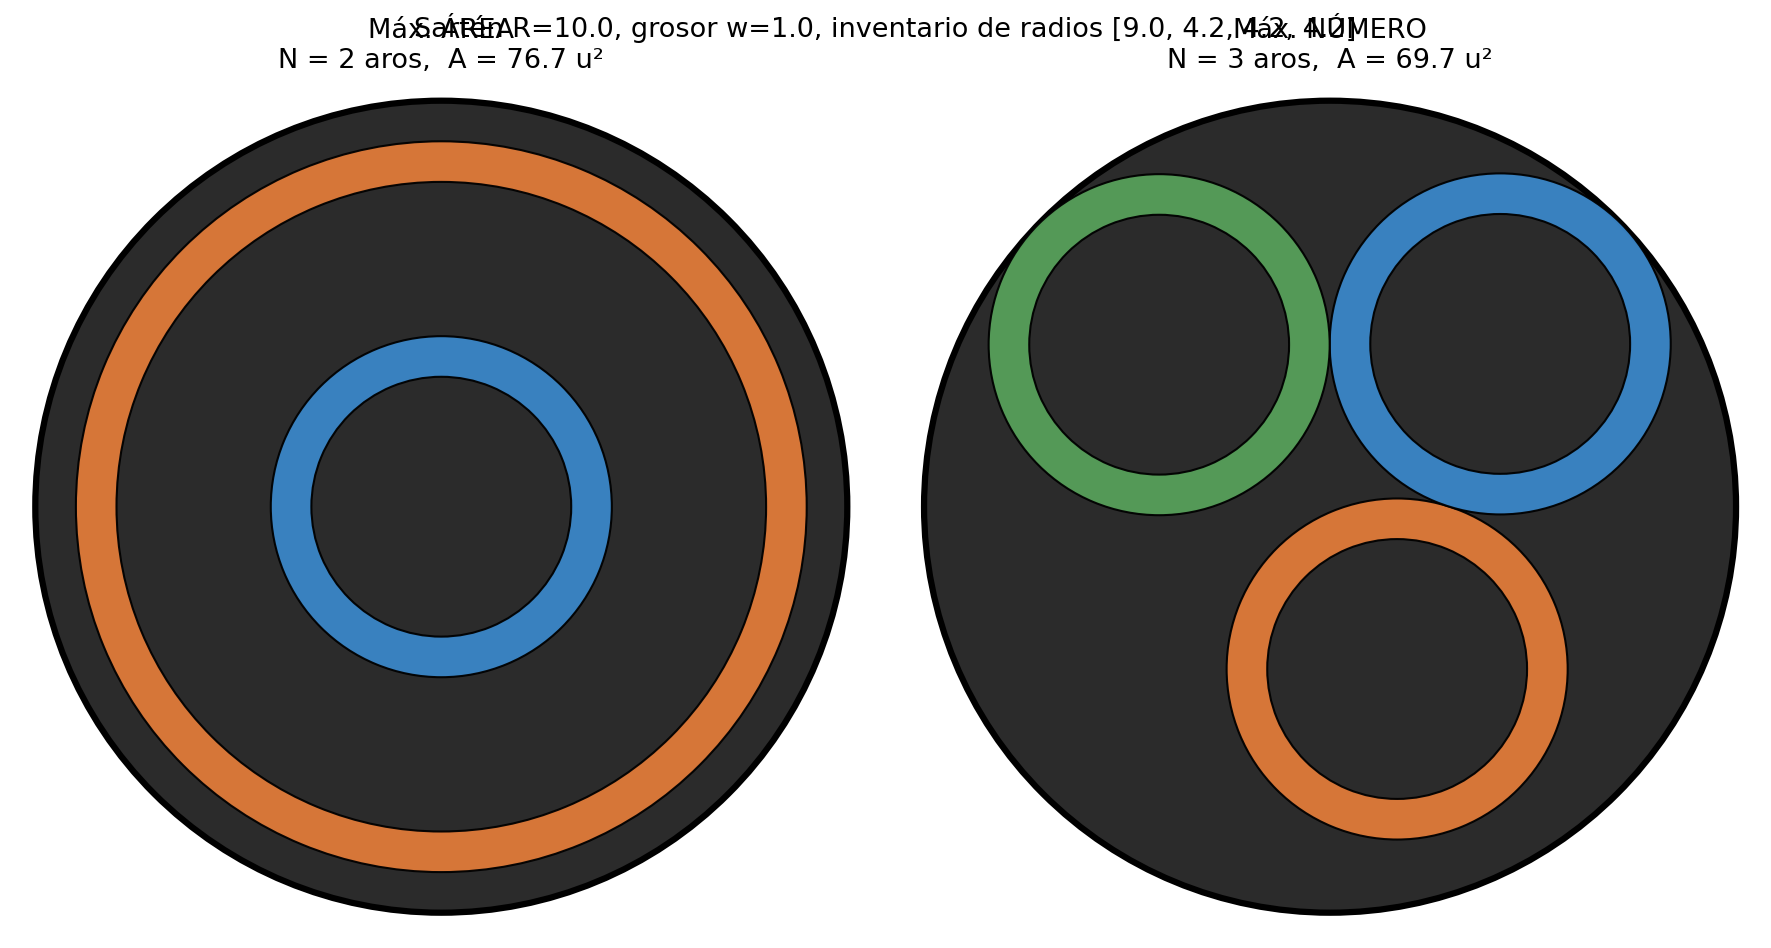
\includegraphics[width=0.72\textwidth]{figures/divergencia_calamares.png}\\[1ex]
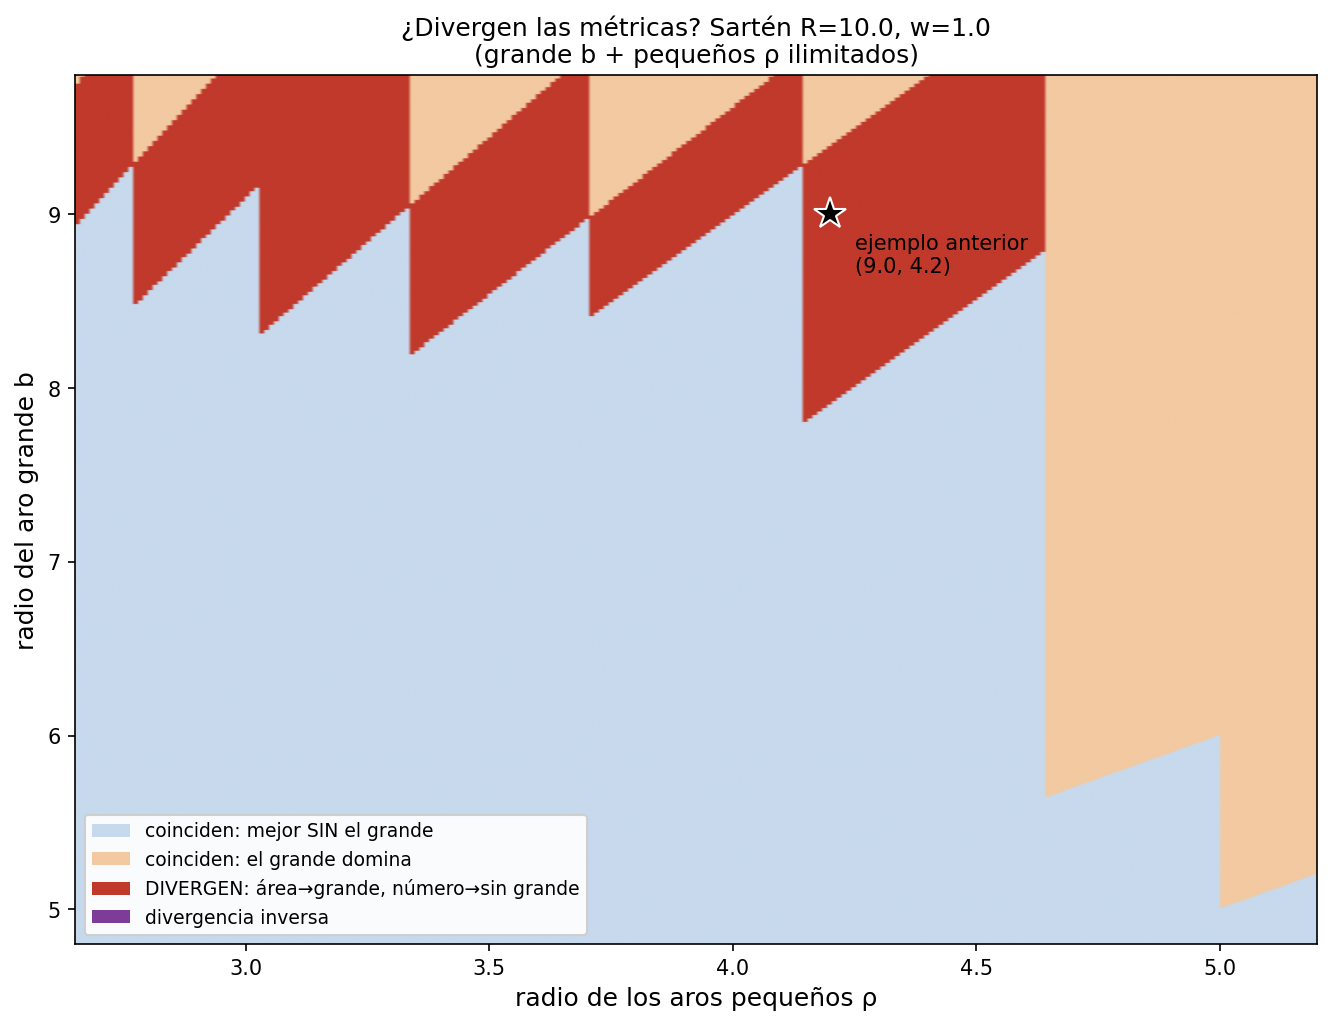
\includegraphics[width=0.72\textwidth]{figures/franja_divergencia.png}
\caption{Top: the minimal divergence instance; area optimum (left) versus
cardinality optimum (right). Bottom: phase diagram of the divergence band for
uniform width.}
\label{fig:phase}
\end{figure}

\begin{figure}[ht]
\centering
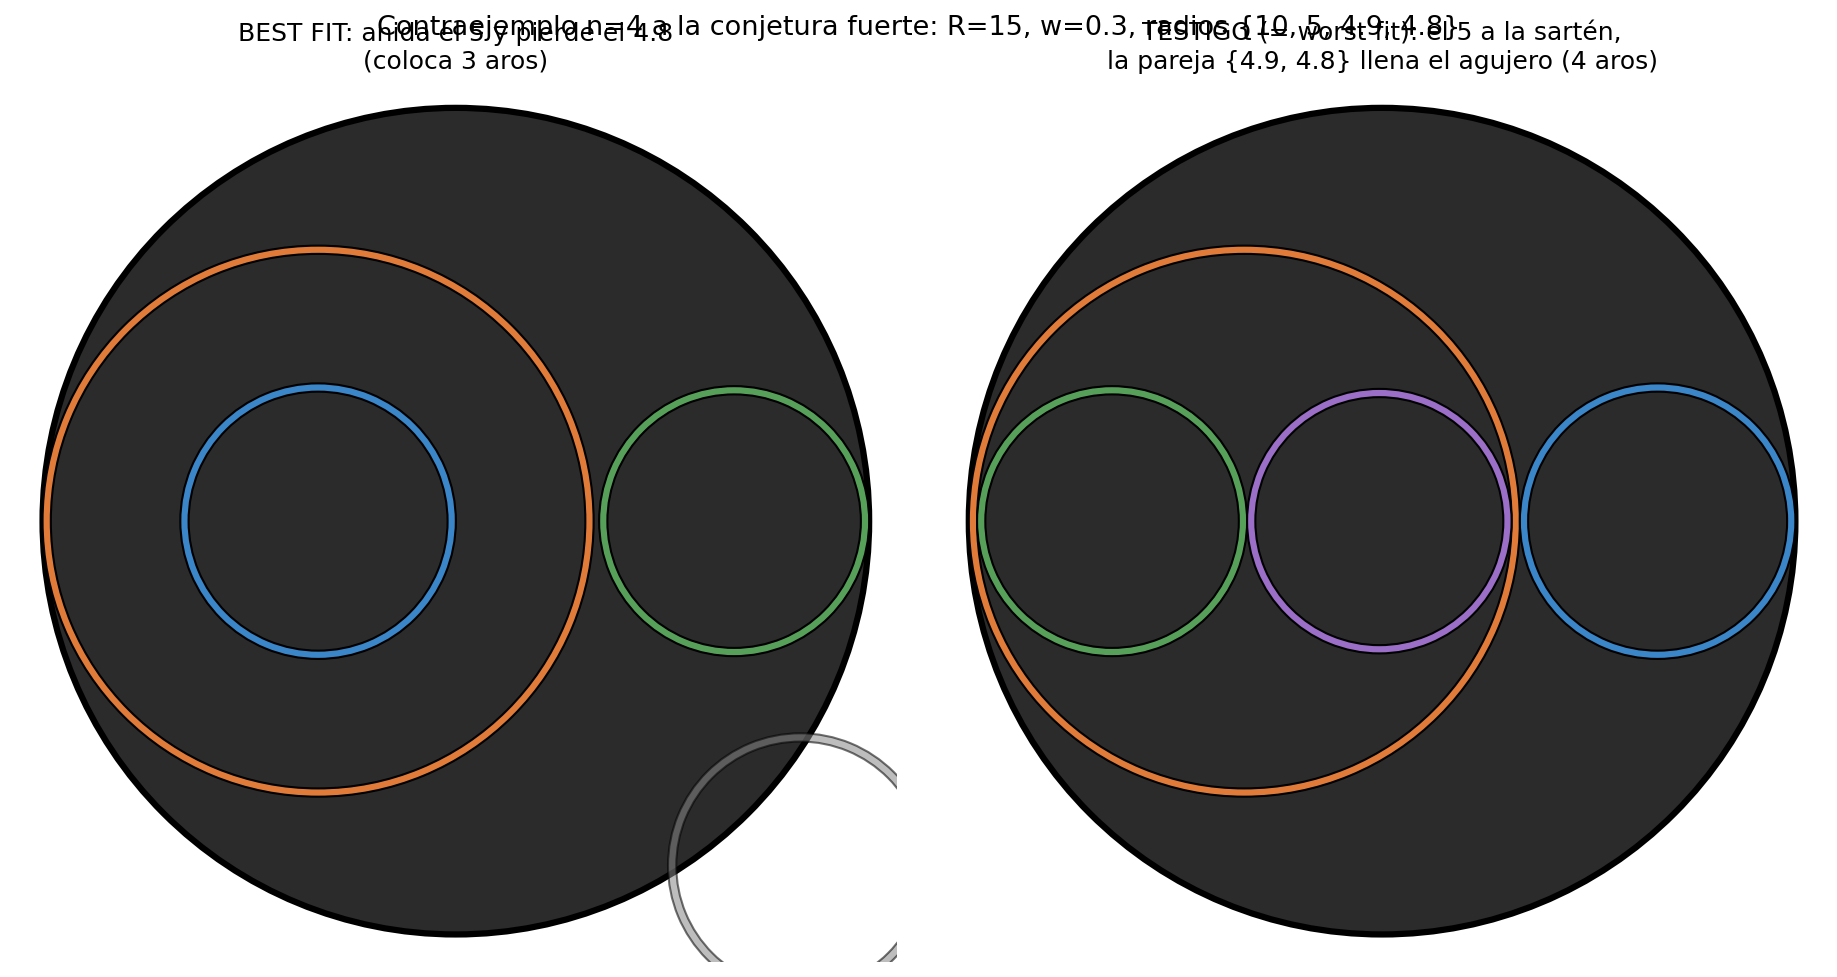
\includegraphics[width=0.8\textwidth]{figures/contraejemplo_n4.png}
\caption{The $n=4$ counterexample of Theorem~\ref{thm:n4}: best fit (left)
nests the $5$ and loses the $4.8$; the witness (right), realized by worst fit,
places all four rings.}
\label{fig:n4}
\end{figure}

\section{Hardness decouples into two layers}\label{sec:hardness}

If all radii lie within a band of width less than $w$, no nesting is
possible and the decision problem ``do all rings fit?'' is exactly circle
packing of the outer radii into the pan.

\paragraph{The geometric layer.}
Since Theorems~\ref{thm:selection} and~\ref{thm:oblivious} hold for
arbitrary containers, our model contains, as the special case of a
\emph{square} pan with a no-nesting band, the problem of deciding whether
given circles fit into a square, which is NP-hard by reduction from
3-\textsc{Partition}~\cite{DemaineFeketeLang2010}; hence the geometric layer
of the model is NP-hard. Membership in NP is itself delicate, because tight
packings may require coordinates without short descriptions -- a phenomenon
made precise by the $\exists\mathbb R$-completeness framework for
two-dimensional packing~\cite{AbrahamsenMiltzowSeiferth2020}. For the disk
pan specifically, we are not aware of a published NP-hardness proof (the
related-work discussions of~\cite{FeketeKeldenichScheffer2019} and its
companions attribute hardness to the square container only), and we leave
its precise status as part of Open Problem~\ref{op:misc}. Integer-programming
formulations for circle packing in rectangular containers are studied
in~\cite{Litvinchev2014}.

\paragraph{The combinatorial layer.}
Independently of the geometry, the \emph{additive surrogate}
(Theorem~\ref{thm:additive}) is weakly NP-hard, and here the reduction can
be made exact despite the per-ring penalty in the area.

\begin{proposition}[The additive layer is weakly NP-hard]
\label{prop:additivehard}
Deciding whether an instance of the additive surrogate admits a feasible
set of contact area at least a given threshold is weakly NP-hard, already
for instances with a no-nesting radius band.
\end{proposition}
\begin{proof}
Reduce from \textsc{Equal-Cardinality Partition}: given positive integers
$a_1,\dots,a_n$, $n$ even, with $\sum_i a_i=2B$, decide whether some $S$
with $|S|=n/2$ has $\sum_{S}a_i=B$. (This variant is NP-hard by the
standard padding: scaling a \textsc{Partition} instance by $2n$ and
adjoining $n$ unit items forces, modulo $2n$, every solution to use exactly
$n$ of the $2n$ items.) Fix any width $w>0$, set $M=3B$, pick
$\delta\in\bigl(\tfrac{w}{3B},\tfrac{w}{2B}\bigr)$, and take radii
$r_i=\delta(a_i+M)$ with pan capacity $R^{+}=\delta\bigl(\tfrac n2M+B\bigr)$.
All radii lie in $[3B\delta,\,5B\delta]$, so $r_i>w$ (each is a genuine
ring, $a(r)=2\pi wr-\pi w^2$) and $r_{\max}-r_{\min}=2B\delta<w$ (no
nesting): feasibility is exactly $\sum_S r_i\le R^{+}$. Write $s=|S|$ and
$t=\sum_S a_i\le 2B$; the area is
$A(S)=2\pi w\delta(sM+t)-\pi w^2 s$, and we ask whether
$A(S)\ge\Theta:=2\pi w\delta\bigl(\tfrac n2M+B\bigr)-\pi w^2\tfrac n2$.
If a balanced partition exists, taking $S$ with $s=n/2$, $t=B$ attains
$\Theta$ exactly. Conversely: $s>n/2$ is infeasible, since it would force
$(s-\tfrac n2)M\le B-t\le B<M$. For $s=\tfrac n2-q$ with $q\ge1$, the
requirement $A(S)\ge\Theta$ rearranges to $wq\ge2\delta(qM+B-t)$, but
\[
2\delta(qM+B-t)\;\ge\;2\delta(qM-B)\;\ge\;2\delta q(M-B)\;=\;4\delta qB
\;>\;wq
\]
using $t\le2B$, $q\ge1$, $M=3B$ and $\delta>\tfrac{w}{4B}$ (implied by
$\delta>\tfrac{w}{3B}$): impossible. Finally $s=n/2$ forces $t\ge B$ from
$A\ge\Theta$ and $t\le B$ from feasibility, i.e.\ $t=B$: a balanced
partition.
\end{proof}

Superincreasing radii eliminate exactly this combinatorial layer --
precisely as in the superincreasing knapsack~\cite{Gupte2016} -- leaving
only the geometric one: by Theorem~\ref{thm:selection}, the area optimum
then reduces to $n$ calls to a sibling-packing feasibility oracle. Useful
blackboxes for the remaining geometry include the critical-density theorem
for disks in a disk (any family of total area at most half the container's
packs, and $1/2$ is tight)~\cite{FeketeKeldenichScheffer2019} and Split
Packing~\cite{FeketeMorrScheffer2019}.

\section{Generalizations}\label{sec:general}

The model invites several generalizations, all of which we record here both as
context for the theorems (two of them hold with no extra work) and as a
research program.

\emph{(a) Container shape and dimension.} Theorems~\ref{thm:selection}
and~\ref{thm:oblivious} are stated and proved for arbitrary containers in
$\R^d$: rectangular griddles, and tubes/spherical shells in three dimensions
-- the original RCPP setting -- are covered verbatim, because the exchange
argument acts inside the vacated ball of the moved ring only. The sharpness
results (Section~\ref{sec:sharp}) are disk-specific; their analogues for
squares and in $\R^3$ are open.

\emph{(b) Variable width.} With per-ring widths $w_i$, a large ring may have a
small hole, which destroys the ``nesting rescue'' and should widen the
divergence band of Section~\ref{sec:divergence} dramatically; the
superadditivity lemma must be re-examined since $a$ depends on both $r$ and
$w$.

\emph{(c) Flexible rings.} Real squid rings bend: a ring partially resting on
another still touches the pan outside the overlap, up to a lifted ramp of
width $\delta$ around each overlap. The idealization $\delta=0$ (contact area
equals the annulus minus the overlapped region) defines a continuous
relaxation in which partial placements trade contact for cardinality; $\delta>0$
penalizes overlaps by a dead band proportional to the overlap perimeter.

\emph{(d) Infinite inventories.} Unlimited supplies (already used in the
phase diagram) suggest degenerate limits: maximal nested chains
$r,\,r-w,\,r-2w,\dots$, density questions, and Apollonian-type limit
configurations.

\emph{(e) Objectives.} Theorem~\ref{thm:selection} covers every positive,
strictly increasing, superadditive value; weighted counts and concave values
fall outside and, by Proposition~\ref{prop:count}, genuinely so.

\section{Open problems}\label{sec:open}

\begin{openproblem}\label{op:assembly}
Prove Conjecture~\ref{conj:tribo} by assembling the universal reinsertion
lemma from the pieces of Sections~\ref{sec:width}--\ref{sec:generic}:
combinatorics ($\rho^*_k=\rho^*_3$, $\omega_c=\omega_T$) below $\omega_T$ and
the wall hierarchy above it. The documented remaining gaps are the width
tips ($j=1$ with $\omega\ge0.9626$; $j=2$ with $\omega\ge0.624$; $j=3$ with
$\omega\ge0.896$), the $\Psi_j$ recursion patch, a quantitative gap lemma
(small rings against the double-pocket wall; tiny $\sigma_2$), profiles with
three or more reinserted pieces beyond the combinatorial bound, and the case
where $u$ is the pan.
\end{openproblem}

\begin{openproblem}\label{op:oracle}
Can a placement rule with access to the full input attain the lex-max set with
polynomially many calls to a sibling-packing oracle, or is there a
complexity-theoretic obstruction?
\end{openproblem}

\begin{openproblem}\label{op:misc}
Characterize the divergence band of Section~\ref{sec:divergence} exactly;
determine the approximability of the cardinality objective; decide whether
the additive surrogate admits a pseudopolynomial algorithm for integer
radii; and settle the complexity of deciding packability of given circles
into a \emph{disk} container (NP-hardness is only published for the square).
\end{openproblem}

\section*{Acknowledgements}
The results of Sections~\ref{sec:threshold}--\ref{sec:generic} were developed
with extensive computer assistance (Anthropic's Claude) under a
draft--verify workflow: every result was independently rederived from its
bare statement by an adversarial verification pass before being accepted,
and several statements were corrected or sharpened by that pass; the reports
are part of the repository. To be explicit about epistemic status: the
mathematical guarantee for every claim is the written proof and, where a
proof delegates an identity, an exact symbolic computation; the verification
workflow and the numerical sweeps are quality control and evidence, never a
substitute for proof.

\appendix
\section{Verification map}\label{app:verifmap}

Every theorem of Sections~\ref{sec:threshold}--\ref{sec:generic} is backed in
the accompanying repository by (i) a self-contained draft with complete
proofs, (ii) a verification script whose blocks separate exact symbolic
identities (\texttt{sympy}) from numerical sweeps, all green, and (iii) an
\emph{adversarial verification report}: an independent rederivation of each
result from its statement alone, followed by an audit and directed attacks.
The correspondence, as ``verified claims (script blocks)'', is:
Theorem~\ref{thm:rigidfloor} -- \texttt{suelo\_rigido}, 10/10 claims
(7 blocks); slack pans and the universal trio frontier --
\texttt{universal} (5/5 blocks); the $\kappa$ identity -- \texttt{h1},
6/6 claims (5/5 blocks); the width curve and Theorem~\ref{thm:corner} --
\texttt{grosor} 8/8 claims, \texttt{esquina} 6/6 claims (5/5 blocks);
profile thresholds -- \texttt{perfil\_tres}, \texttt{cuatro}
(\texttt{cuatrok} 5/5 blocks); the corona criterion -- \texttt{corona}
(5/5 blocks); occupant walls, the opposite-disk lemma and the metallic
floors -- \texttt{ocupantes} (5/5), \texttt{bloqueadores} (6/6); the
double-pocket wall and the golden line -- \texttt{bolsillo} (6/6). Several
statements were corrected or sharpened by the adversarial round (a missing
hypothesis in the trio frontier, a refuted ``leak'' family, the
$\alpha\ge o_1$ case split); the reports record each incident.

\section{Complete proof of Theorem~\ref{thm:rigidfloor}}\label{app:rigidproof}

Throughout, work in the normalization of Theorem~\ref{thm:rigidfloor}:
$r_1=1$, $t=r_2$, $u=r_3$, $v=r_4$, width $\omega>0$, pan radius $R=1+t$,
and recall $b(t)=t(1+t)/(1+t+t^2)$, $T^3=T^2+T+1$, $t^{*}=1/T$
(equivalently $t^{*3}+t^{*2}+t^{*}=1$), $\varphi=(1+\sqrt5)/2$. All exact
algebraic identities used below are additionally verified in
\texttt{code/rigido.py} (block V5).

\begin{lemma}[Half-angle identity]\label{lem:S1}
Let two circles of radii $a,b$ be internally tangent to the wall of a disk
of radius $R$ (centers at distances $R-a$, $R-b$ from the center). If
$a+b\le R$, the minimal angular separation $\theta(a,b)$ guaranteeing
disjoint interiors is well defined, lies in $[0,\pi]$, satisfies
\[
\sin^2\tfrac{\theta(a,b)}2=f(a)f(b),\qquad f(x)=\frac{x}{R-x},
\]
and is increasing in each argument; two wall-tangent circles at angular
separation $\gamma$ have disjoint interiors iff $\gamma\ge\theta(a,b)$.
\end{lemma}
\begin{proof}
By the law of cosines the center distance
$D(\gamma)^2=(R-a)^2+(R-b)^2-2(R-a)(R-b)\cos\gamma$ is increasing on
$[0,\pi]$, and disjointness is $D\ge a+b$. At the threshold,
$1-\cos\theta=\bigl[(a+b)^2-(a-b)^2\bigr]/\bigl(2(R-a)(R-b)\bigr)
=2ab/\bigl((R-a)(R-b)\bigr)$, i.e.\
$\sin^2(\theta/2)=f(a)f(b)$; and $f(a)f(b)\le1$ is exactly $a+b\le R$.
Monotonicity is that of $f$.
\end{proof}

\begin{lemma}[Construction]\label{lem:S2}
Let $v\le u\le t<1$ and $R=1+t$. If
$\theta(1,u)+\theta(1,v)+\theta(u,v)\le2\pi$, then $\{1,u,v\}$ packs in the
disk of radius $R$.
\end{lemma}
\begin{proof}
All three angles are defined ($1+u\le R\iff u\le t$, and $u+v\le2t<R$).
Place the three circles wall-tangent with the unit circle in the middle:
centers at angles $0$, $+\theta(1,u)$, $-\theta(1,v)$. Each circle is
contained in the disk (internal wall tangency). The pairs $(1,u)$ and
$(1,v)$ are separated by exactly their thresholds. For $(u,v)$, the angular
difference is $\Delta=\theta(1,u)+\theta(1,v)$ and the separation is
$\gamma=\min(\Delta,2\pi-\Delta)$. If $\gamma=\Delta$: by monotonicity
(Lemma~\ref{lem:S1}, $1\ge u$), $\theta(1,v)\ge\theta(u,v)$, so
$\Delta\ge\theta(u,v)$. If $\gamma=2\pi-\Delta$: the hypothesis gives
$2\pi-\Delta\ge\theta(u,v)$.
\end{proof}

\begin{lemma}[Algebraic reduction]\label{lem:S3}
Define $\psi(x)=\sqrt{(t-x)/x}$ (decreasing, $\psi(t)=0$) and
$\tau=t/\sqrt{1+t}$; note the exact identities $\psi(b(t))=\tau$ and
$t/(1+\tau^2)=b(t)$. If $v\le u\le t<1$ and $\psi(u)+\psi(v)\ge\tau$, then
$\theta(1,u)+\theta(1,v)+\theta(u,v)\le2\pi$, and hence $\{1,u,v\}$ packs
in the disk $R=1+t$ by Lemma~\ref{lem:S2}.
\end{lemma}
\begin{proof}
Let $A=\sqrt{f(1)f(u)}$, $B=\sqrt{f(1)f(v)}$, $C=\sqrt{f(u)f(v)}$ (the
sines of the half-angles); the goal is
$\arcsin A+\arcsin B+\arcsin C\le\pi$. If $\arcsin A+\arcsin B\le\pi/2$
there is nothing to prove, since $\arcsin C\le\pi/2$. Otherwise the goal is
equivalent, both sides lying in $[0,\pi/2]$, to
$C\le\sin(\arcsin A+\arcsin B)=A\sqrt{1-B^2}+B\sqrt{1-A^2}$. Dividing by
$C>0$ and writing $G(x)=f(1)/f(x)-f(1)^2$,
\[
\frac{A\sqrt{1-B^2}}{C}=\sqrt{G(v)},\qquad
\frac{B\sqrt{1-A^2}}{C}=\sqrt{G(u)},\qquad
G(x)=\frac{(1+t)(t-x)}{t^2x},
\]
the last identity by direct computation with $f(1)=1/t$,
$f(x)=x/(1+t-x)$; the radicals are real because $f(1)f(x)\le1\iff x\le t$.
Thus $\sqrt{G(x)}=\bigl(\sqrt{1+t}/t\bigr)\psi(x)$ and, by hypothesis,
$\sqrt{G(u)}+\sqrt{G(v)}=\bigl(\sqrt{1+t}/t\bigr)(\psi(u)+\psi(v))
\ge\bigl(\sqrt{1+t}/t\bigr)\tau=1$, which is the required inequality.
\end{proof}

The contrapositive used below: hypothesis (F3) implies
$\psi(u)+\psi(v)<\tau$. This is the only direction ever used -- the
\emph{constructive} one -- so no exactness of any angular criterion is
assumed anywhere in this appendix.

\begin{lemma}[Corner minimization]\label{lem:S4}
Let $0<v\le u\le t<1$ with $\psi(u)+\psi(v)<\tau$. Then:
\textup{(1)} $u,v>b(t)$;
\textup{(2)} if $t\ge1/\varphi$ then $u+v>1$;
\textup{(3)} if $t<1/\varphi$ then $u+v>t+b(t)$.
\end{lemma}
\begin{proof}
(1) Each summand is $<\tau$, $\psi$ is decreasing and $\psi(b(t))=\tau$.
(2) $u+v>2b(t)$ and $2b(t)-1=(t^2+t-1)/(t^2+t+1)\ge0$ exactly when
$t\ge1/\varphi$.
(3) Substitute $\alpha=\psi(u)$, $\beta=\psi(v)$, so $u=U(\alpha)$,
$v=U(\beta)$ with $U(z)=t/(1+z^2)$ strictly decreasing; the region is
$\alpha,\beta\ge0$, $\alpha+\beta<\tau$. Increasing $\alpha$ to
$\tau-\beta$ decreases $u$, so $u+v>U(\tau-\beta)+U(\beta)=:W(\tau-\beta)$.
Now $U''(z)=2t(3z^2-1)/(1+z^2)^3\le0$ for $z\le1/\sqrt3$, and
$\tau\le1/\sqrt3\iff3t^2-t-1\le0\iff t\le(1+\sqrt{13})/6=0.7676\dots$,
which covers $t<1/\varphi=0.618\dots$ with room to spare. Hence $U$ is
concave on $[0,\tau]$, $W$ is concave, and its minimum over $[0,\tau]$ is
at the endpoints: $W\ge W(0)=U(0)+U(\tau)=t+t/(1+\tau^2)=t+b(t)$, by the
identity $t/(1+\tau^2)=b(t)$.
\end{proof}

\begin{proof}[Proof of the strict floor in Theorem~\ref{thm:rigidfloor}]
Let $I\in\mathcal F$, normalized. By (F3) and the contrapositive of
Lemmas~\ref{lem:S2}--\ref{lem:S3}, $\psi(u)+\psi(v)<\tau$. If
$t\ge1/\varphi$, Lemma~\ref{lem:S4}(2) gives $u+v>1$, contradicting (F2)
($u+v\le1-\omega<1$); so $t<1/\varphi$ and Lemma~\ref{lem:S4}(3) gives the
blocking pressure $u+v>t+b(t)$. Chaining with the witness pressure (F2),
\[
t+b(t)\;<\;u+v\;\le\;1-\omega\;<\;1,
\]
and $t+b(t)<1\iff t(1+t)<(1-t)(1+t+t^2)=1-t^3\iff t^3+t^2+t<1\iff t<t^{*}$
(which also proves that $\mathcal F$ forces $t<t^{*}$). Finally
\[
\rho\;\ge\;\rho_2=\frac{u+v}{t}\;>\;\frac{t+b(t)}{t}
\;=\;1+\frac{1+t}{1+t+t^2}\;=:\;L(t),
\]
and $L$ is strictly decreasing ($L'=-(t^2+2t)/(1+t+t^2)^2<0$) with
$L(t^{*})=1/t^{*}=T$ (an identity modulo $t^{*3}+t^{*2}+t^{*}=1$). Since
$t<t^{*}$: $\rho>L(t)>L(t^{*})=T$.
\end{proof}

It remains to prove exactness of the infimum. Two ingredients: the rigid
pocket is exact, and infeasibility survives small perturbations.

\begin{proposition}[Exact rigid pocket]\label{prop:S5}
For $0<v\le t<1$, the triple $\{1,t,v\}$ packs in the disk of radius
$R=1+t$ if and only if $v\le b(t)$.
\end{proposition}
\begin{proof}
\emph{Rigidity.} Centers satisfy $|c_1|\le t$, $|c_t|\le1$ and
$|c_1-c_t|\ge1+t$; the triangle inequality forces equality throughout, so
up to rotation $c_1=(-t,0)$, $c_t=(1,0)$.
\emph{Sufficiency.} The pocket circle tangent to the wall and to both has
radius $b(t)$; any $v\le b(t)$ placed concentrically inside it works.
\emph{Necessity.} Let $X$ be the center of $v$, $d=|X|>0$, and $\gamma$ the
angle between $X$ and $(1,0)$. Disjointness reads
$d^2+t^2+2dt\cos\gamma\ge(1+v)^2$ and $d^2+1-2d\cos\gamma\ge(t+v)^2$, which
bound $\cos\gamma$ from below and above; compatibility of the two bounds
requires $(1+t)d^2\ge(1+v)^2+t(t+v)^2-t(1+t)$, and with $d\le R-v=1+t-v$:
\[
(1+t)(1+t-v)^2-(1+v)^2-t(t+v)^2+t(1+t)\;\ge\;0 .
\]
The left-hand side factors \emph{exactly} as
$4\,(t^2+t+1)\,\bigl(b(t)-v\bigr)$ (symbolic identity, V5), whence
$v\le b(t)$.
\end{proof}

\begin{lemma}[Closure and monotonicity of packability]\label{lem:S6a}
Let $D=\{(t,u,v):0<v\le u\le t<1\}$ and say $p=(t,u,v)$ \emph{packs} if
there are centers with $|c_1|\le t$, $|c_2|\le1+t-u$, $|c_3|\le1+t-v$,
$|c_1-c_2|\ge1+u$, $|c_1-c_3|\ge1+v$, $|c_2-c_3|\ge u+v$. Let
$E\subseteq D$ be the packable set. Then:
\textup{(1)} $E$ is downward closed in $(u,v)$;
\textup{(2)} $E$ is closed in $D$;
\textup{(3)} for fixed $t,v$, the set $\{u\in[v,t]:(t,u,v)\in E\}$ is empty
or a closed interval $[v,u_{\max}]$ with the maximum attained; in
particular, if $(t,t,v)\notin E$, then $(t,u,v)\notin E$ for all
$u\in(u_{\max},t]$ -- the infeasibility of the rigid corner propagates to
$\delta:=t-u\in[0,\delta_0)$, $\delta_0=t-u_{\max}>0$.
\end{lemma}
\begin{proof}
(1) The same centers witness (all six constraints relax). (2) Witness
centers live in a fixed compact ball; take a convergent subsequence of
witnesses along $p_k\to p$ and pass to the limit in the six non-strict
continuous constraints. (3) By (1) the set is an initial segment, by (2) it
is closed.
\end{proof}

\begin{proposition}[The infimum is $T$ and is not attained]\label{prop:S6}
$\inf\{\rho(I):I\in\mathcal F\}=T$.
\end{proposition}
\begin{proof}
$\ge$ and non-attainment: the strict floor above. $\le$: fix $t<t^{*}$, set
$\varepsilon_t=(1-t-b(t))/2>0$ and
$v_t=b(t)+\min\bigl(\varepsilon_t,(t-b(t))/2\bigr)$. By
Proposition~\ref{prop:S5}, $(t,t,v_t)$ is infeasible; by
Lemma~\ref{lem:S6a}(3) there is $\delta\in(0,\min(\varepsilon_t,t-v_t))$
with $(t,t-\delta,v_t)$ infeasible. The instance
$I_t=(1,\,t,\,t-\delta,\,v_t)$ with $\omega=1-(t-\delta+v_t)>0$ satisfies
(F1)--(F3) and the strict orderings, so $I_t\in\mathcal F$, and
$\rho(I_t)=\rho_2\le\bigl(t+b(t)+\varepsilon_t\bigr)/t
=L(t)+\varepsilon_t/t\longrightarrow L(t^{*})=T$ as $t\to t^{*}$
(the other tails are smaller: $\rho_1=t+u+v<3t<T$ and $\rho_3=v/u<1$).
\end{proof}

\begin{proof}[Proof of Remark~\ref{rem:slack}]
A packing in a disk of radius $R'\le R$ is a packing in the disk of radius
$R$ (translate to concentric position; containment is preserved, pairwise
constraints are unchanged). Hence non-packability at radius $R$ implies
non-packability at radius $r_1+r_2\le R$, so an instance with a slack pan
satisfying (F2) and (F3) at its own radius satisfies (F2)--(F3) at radius
$r_1+r_2$, and the floor applies verbatim; the approximating family of
Proposition~\ref{prop:S6} has $R=r_1+r_2$, which is admissible, so the
infimum is unchanged.
\end{proof}

\section{Verification details for Theorem~\ref{thm:twins}}\label{app:verif}

All feasibilities in the twin instances are two-circle-exact except three
facts, proved here; every numerical claim is also reproduced by the scripts in
the repository (\texttt{code/gemelas.py}).

\paragraph{(V1) $\{10,\,4.99,\,4.50\}$ does not pack in a disk of radius 15.}
As in Lemma~\ref{lem:cap}: $|c_A|\le5$, $|c_X|\le10.01$, $|c_Y|\le10.5$,
$|c_A-c_X|\ge14.99$, $|c_A-c_Y|\ge14.5$, $|c_X-c_Y|\ge9.49$; the first two
give $a:=|c_A|\ge4.98$. With $u=-c_A/|c_A|$,
$c_X\!\cdot\!u\ge(124.5-a^2)/(2a)\ge9.95$ and
$c_Y\!\cdot\!u\ge(100-a^2)/(2a)\ge7.5$ (both decreasing in $a$, evaluated at
$a=5$), with transverse norms at most
$\sqrt{10.01^2-9.95^2}\le1.095$ and $\sqrt{10.5^2-7.5^2}\le7.349$.
Hence $|c_X-c_Y|^2\le10.01^2+10.5^2-2(9.95\cdot7.5-1.095\cdot7.349)
\le77.30$, so $|c_X-c_Y|\le8.80<9.49$.

\paragraph{(V2) With the pan pair $\{10,5\}$ placed, no third circle of radius
$z\in\{4.74,4.76\}$ fits.}
From $|c_A|\le5$, $|c_B|\le10$ and $|c_A-c_B|\ge15$ the triangle inequality
forces equalities: the pair is diametrically rigid, $c_B=10u$ for a unit
vector $u$ and $c_A=-5u$. For a third circle of radius $z$:
$c_z\!\cdot\!u\ge\bigl((10{+}z)^2-(15{-}z)^2-25\bigr)/10$, which equals $8.8$
for $z=4.76$ and $8.7$ for $z=4.74$; then
$|c_z-c_B|^2=|c_z|^2-20\,c_z\!\cdot\!u+100\le(15-z)^2-20\,c_z\!\cdot\!u+100$,
giving $|c_z-c_B|\le5.38<9.76$ and $\le5.60<9.74$ respectively.

\paragraph{(V3) $\{10,\,4.76,\,4.74\}$ packs in a disk of radius 15.}
Explicit boundary configuration:
$c_A=(-5,0)$,
$c_X=10.24(\cos30.77^\circ,\ \sin30.77^\circ)\approx(8.799,\,5.238)$,
$c_Y=10.26(\cos32.02^\circ,\ -\sin32.02^\circ)\approx(8.700,\,-5.440)$.
Then $|c_A|=5$, $|c_X|=10.24=15-4.76$, $|c_Y|=10.26=15-4.74$ (all inside);
$|c_A-c_X|=14.76$ and $|c_A-c_Y|=14.74$ (exact tangencies, chosen via the
boundary angles); and $|c_X-c_Y|\approx10.68\ge9.50$ with ample margin.

\paragraph{(V4) Hole facts.} The hole of the $10$ has radius $9.495$;
$4.99+4.50=9.49\le9.495$ (the pair fits, two-circle exact) while
$4.76+4.74=9.50>9.495$ and $5+4.50=9.50>9.495$ (blocked, two-circle exact).

\begin{thebibliography}{99}

\bibitem{PedrosoCunhaTavares2016}
J.~P. Pedroso, S.~Cunha, J.~N. Tavares.
Recursive circle packing problems.
\emph{International Transactions in Operational Research} 23(1--2):355--368,
2016.

\bibitem{Gleixner2020}
A.~Gleixner, S.~J. Maher, B.~M\"uller, J.~P. Pedroso.
Price-and-verify: a new algorithm for recursive circle packing using
Dantzig--Wolfe decomposition.
\emph{Annals of Operations Research} 284(2):527--555, 2020.

\bibitem{CoffmanGareyJohnson1987}
E.~G. Coffman~Jr., M.~R. Garey, D.~S. Johnson.
Bin packing with divisible item sizes.
\emph{Journal of Complexity} 3(4):406--428, 1987.

\bibitem{DemaineFeketeLang2010}
E.~D. Demaine, S.~P. Fekete, R.~J. Lang.
Circle packing for origami design is hard.
In \emph{Origami$^5$: Proc.\ 5th International Conference on Origami in
Science, Mathematics and Education}, A K Peters, 2011, pp.\ 609--626.

\bibitem{FeketeKeldenichScheffer2019}
S.~P. Fekete, P.~Keldenich, C.~Scheffer.
Packing disks into disks with optimal worst-case density.
In \emph{Proc.\ 35th International Symposium on Computational Geometry (SoCG)},
LIPIcs 129, 35:1--35:19, 2019. Journal version:
\emph{Discrete \& Computational Geometry} 69:51--90, 2023.

\bibitem{AbrahamsenMiltzowSeiferth2020}
M.~Abrahamsen, T.~Miltzow, N.~Seiferth.
Framework for $\exists\mathbb R$-completeness of two-dimensional packing
problems.
In \emph{Proc.\ 61st IEEE Annual Symposium on Foundations of Computer
Science (FOCS)}, pp.\ 1014--1021, 2020.

\bibitem{FeketeMorrScheffer2019}
S.~P. Fekete, S.~Morr, C.~Scheffer.
Split packing: algorithms for packing circles with optimal worst-case density.
\emph{Discrete \& Computational Geometry} 61(3):562--594, 2019.

\bibitem{GLNO1998}
R.~L. Graham, B.~D. Lubachevsky, K.~J. Nurmela, P.~R.~J. \"Osterg\aa rd.
Dense packings of congruent circles in a circle.
\emph{Discrete Mathematics} 181:139--154, 1998.

\bibitem{Pirl1969}
U.~Pirl.
Der Mindestabstand von $n$ in der Einheitskreisscheibe gelegenen Punkten.
\emph{Mathematische Nachrichten} 40:111--124, 1969.

\bibitem{Melissen1994}
H.~Melissen.
Densest packings of eleven congruent circles in a circle.
\emph{Geometriae Dedicata} 50:15--25, 1994.

\bibitem{Fodor1999}
F.~Fodor.
The densest packing of 19 congruent circles in a circle.
\emph{Geometriae Dedicata} 74:139--145, 1999.

\bibitem{EkanayakeLaFountain2024}
D.~B. Ekanayake, D.~J. LaFountain.
Tight partitions for packing circles in a circle.
\emph{Italian Journal of Pure and Applied Mathematics} 51:115--136, 2024.

\bibitem{Edmonds1971}
J.~Edmonds.
Matroids and the greedy algorithm.
\emph{Mathematical Programming} 1:127--136, 1971.

\bibitem{KorteHausmann1978}
B.~Korte, D.~Hausmann.
An analysis of the greedy heuristic for independence systems.
\emph{Annals of Discrete Mathematics} 2:65--74, 1978.

\bibitem{Gupte2016}
A.~Gupte.
Convex hulls of superincreasing knapsacks and lexicographic orderings.
\emph{Discrete Applied Mathematics} 201:150--163, 2016.

\bibitem{Litvinchev2014}
I.~Litvinchev, L.~Infante, E.~L. Ozuna Espinosa.
Approximate circle packing in a rectangular container: integer programming
formulations and valid inequalities.
In \emph{Computational Logistics (ICCL 2014)}, LNCS 8760, Springer, 2014,
pp.\ 47--60.

\end{thebibliography}

\end{document}
